\subsection*{(e) Stabilitas}
Clustering akhir diulang \TtigaNRun{} kali pada subsampel 80\% yang berbeda, lalu setiap hasil di-\textit{predict} ke seluruh data.
ARI antar run: rata-rata \TtigaStabMean{} (simpangan baku \TtigaStabStd, minimum \TtigaStabMin). Jaccard terendah per cluster \TtigaJaccardMin{}
(Tabel~\ref{tab:t3_stabilitas}, Gambar~\ref{fig:t3stab}), sehingga semua segmen muncul konsisten.

\begin{table}[ht]
\centering\small
\resizebox{\ifdim\width>\linewidth\linewidth\else\width\fi}{!}{%
\begin{tabular}{rlrrrr}
\toprule
k & metode & n\_run & ARI\_mean & ARI\_std & ARI\_min \\
\midrule
7 & kmeans & 6 & 0.984 & 0.004 & 0.973 \\
8 & kmeans & 20 & 0.985 & 0.005 & 0.970 \\
9 & kmeans & 6 & 0.888 & 0.136 & 0.690 \\
\bottomrule
\end{tabular}
}
\caption{Stabilitas: ARI antar run subsampling 80\% (20 run untuk k=8).}
\label{tab:t3_stabilitas}
\end{table}

\begin{figure}[ht]\centering
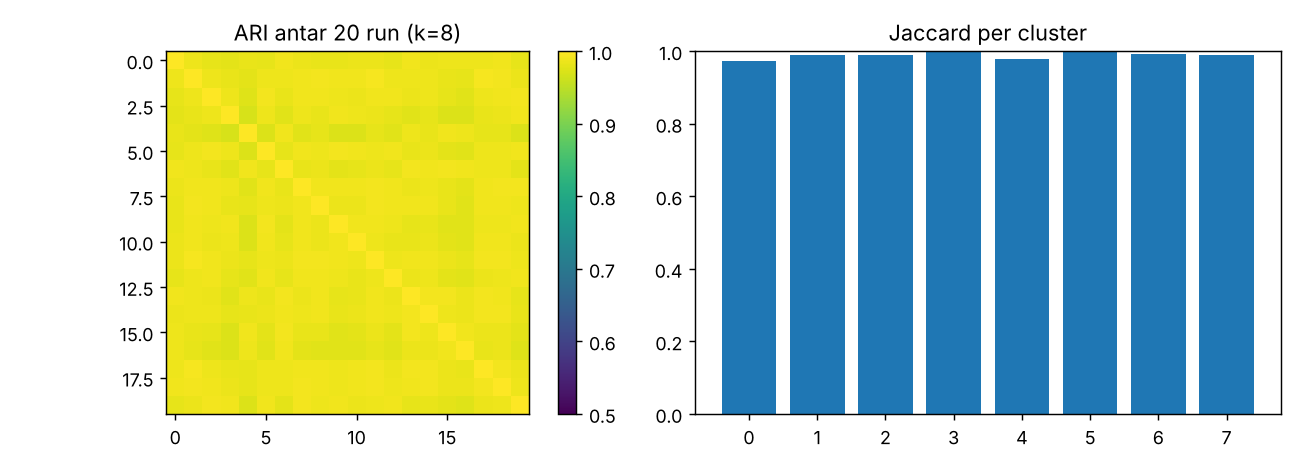
\includegraphics[width=.8\linewidth]{t3_stabilitas.png}
\caption{Kiri: ARI antar run. Kanan: Jaccard tiap cluster terhadap pasangan terdekat di run lain.}\label{fig:t3stab}
\end{figure}

\subsection*{(f) Profil segmen dan aksi marketing}
Terdapat \TtigaNSegmen{} segmen (di luar anomali). Profil median pada fitur asli ada di Tabel~\ref{tab:t3_profil} dan pola pembedanya di Gambar~\ref{fig:t3heat}.
Nama dan aksi per segmen (Tabel~\ref{tab:t3_aksi}) diturunkan dari fitur yang paling membedakan segmen tersebut dari populasi.
Nama segmen hasil otomatis kami cocokkan dengan Tabel~\ref{tab:t3_profil}; dua nama kami ubah agar sesuai profil (segmen~5 menjadi \emph{Pelanggan Loyal Bernilai Tinggi} karena frekuensi dan nilai belanjanya tertinggi, segmen~2 menjadi \emph{Mulai Pasif}). Alasan aksi per segmen: segmen~0 paling sering membeli saat flash sale (69\%), sehingga voucher dengan minimum belanja sedikit di atas keranjangnya dapat menaikkan nilai transaksi; segmen~1 dominan berbelanja pagi hari, sehingga promo dan pengingat dikirim sebelum jam kerja; segmen~2 baru terakhir belanja rata-rata 44 hari lalu, sehingga perlu win-back sebelum benar-benar berhenti; segmen~3 memakai paylater paling tinggi (62\%) di kategori fashion yang rawan retur, sehingga panduan ukuran dan ulasan dapat menekan retur; segmen~4 hampir seluruhnya pengguna iOS dengan belanja besar (Rp3{,}4 juta), cocok untuk produk premium; segmen~5 sudah loyal, sehingga fokusnya menambah nilai lewat cross-sell, bukan diskon; segmen~6 tidak bertransaksi dalam 90 hari, sehingga perlu reaktivasi dengan voucher comeback.
\begin{table}[ht]
\centering\small
\resizebox{\ifdim\width>\linewidth\linewidth\else\width\fi}{!}{%
\begin{tabular}{rrrrrrrlll}
\toprule
segmen & ukuran\_\% & frekuensi\_90h & belanja\_90h (ribu Rp) & recency\_hari & persen\_paylater & persen\_flash\_sale & kategori\_dominan & jam\_dominan & perangkat\_dominan \\
\midrule
0 & 22.70 & 7.00 & 706.60 & 9.20 & 0.17 & 0.69 & fashion & malam & android (74\%) \\
1 & 17.16 & 11.00 & 2690.90 & 6.50 & 0.11 & 0.21 & makanan\_minuman & pagi & android (91\%) \\
2 & 16.63 & 2.00 & 350.55 & 44.20 & 0.17 & 0.30 & makanan\_minuman & sore & android (70\%) \\
3 & 15.52 & 7.00 & 1005.70 & 9.30 & 0.62 & 0.58 & fashion & malam & android (74\%) \\
4 & 14.48 & 8.00 & 3421.80 & 7.50 & 0.10 & 0.17 & makanan\_minuman & siang & ios (96\%) \\
5 & 7.84 & 27.00 & 6741.35 & 6.60 & 0.12 & 0.25 & makanan\_minuman & pagi & android (66\%) \\
6 & 5.67 & 0.00 & 0.00 & 38.50 & 0.17 & 0.33 & makanan\_minuman & malam & android (68\%) \\
\bottomrule
\end{tabular}
}
\caption{Profil segmen (median fitur asli).}
\label{tab:t3_profil}
\end{table}

\begin{table}[ht]
\centering\small
\begin{tabular}{rp{0.23\linewidth}p{0.52\linewidth}}
\toprule
segmen & nama & aksi marketing \\
\midrule
0 & Pemburu Voucher \& Pemburu Flash Sale & voucher bertarget dengan minimum belanja sedikit di atas rata-rata keranjangnya \\
1 & Belanja Pagi \& Pengguna Android & promo pagi hari dan pengingat keranjang sebelum jam kerja \\
2 & Mulai Pasif \& Setia COD & kampanye win-back dengan voucher terbatas waktu \\
3 & Sering Retur \& Pengguna Paylater & panduan ukuran/ulasan produk dan rekomendasi yang lebih akurat \\
4 & Pengguna iOS \& Usia Matang & kampanye produk premium di aplikasi iOS \\
5 & Cepat Membeli \& Rajin Mengulas & rekomendasi produk pelengkap (cross-sell) \\
6 & Pelanggan Tidur & kampanye reaktivasi: voucher comeback + pengingat kategori favorit \\
\bottomrule
\end{tabular}
\caption{Nama segmen dan usulan aksi marketing.}
\label{tab:t3_aksi}
\end{table}

\begin{figure}[ht]\centering
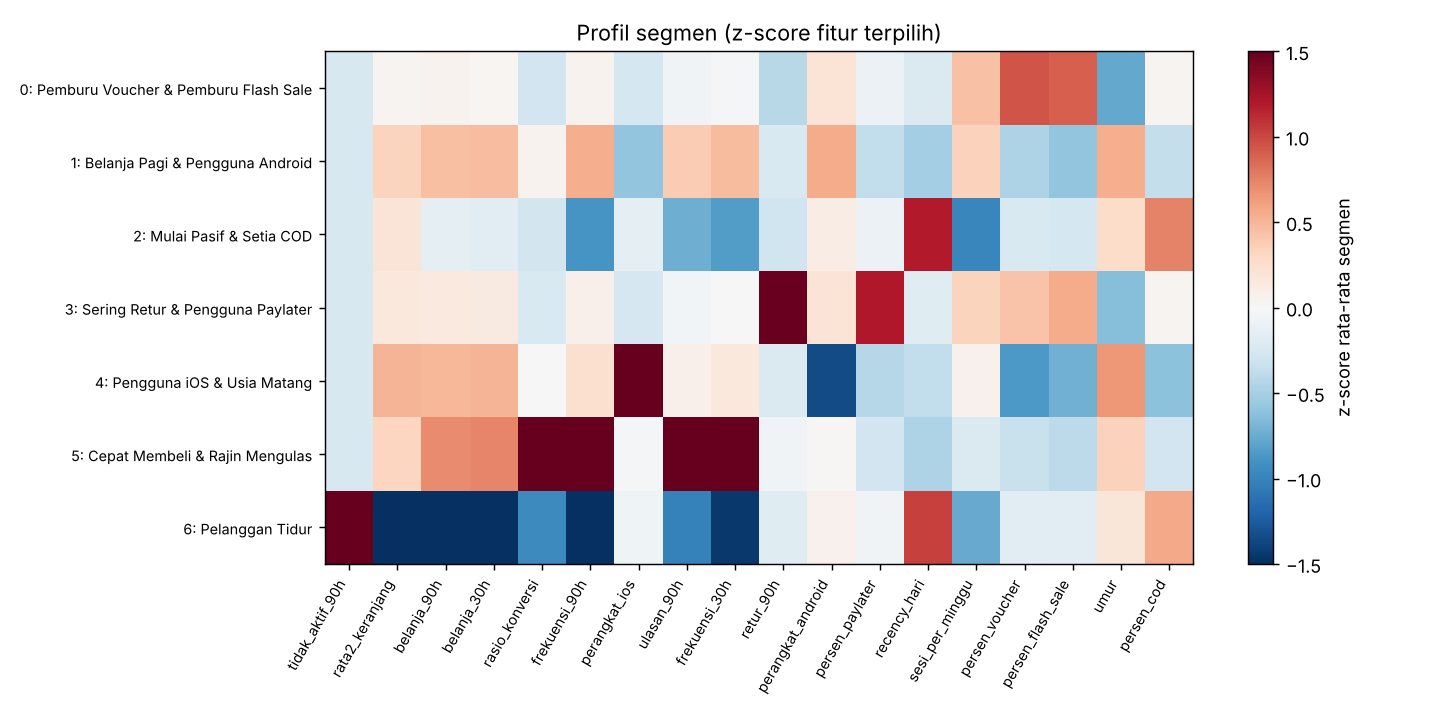
\includegraphics[width=.9\linewidth]{t3_profil_heatmap.png}
\caption{Z-score rata-rata fitur pembeda per segmen.}\label{fig:t3heat}
\end{figure}

\subsection*{(g) Anomali}
Pelanggan diberi label $-1$ bila perilakunya tidak mungkin atau tidak wajar untuk manusia --- lebih dari 100 sesi per minggu (±14 sesi per hari),
rasio konversi > 1, atau belanja 30 hari melebihi belanja 90 hari --- atau bila termasuk cluster yang mayoritas anggotanya melanggar aturan tersebut
(cluster berprofil bot: ratusan sesi per minggu dengan konversi hampir nol). Total \TtigaAnomaliN{} pelanggan (\TtigaAnomaliPersen\%).
Isolation Forest, likelihood GMM, dan jarak ke centroid dibandingkan sebagai alternatif (Tabel~\ref{tab:t3_anomali}); irisannya dengan aturan domain kecil,
artinya detektor statistik umum lebih banyak menandai pelanggan yang sekadar ekstrem namun wajar. Karena pelanggan normal yang diberi $-1$
menurunkan ARI, kami memilih definisi yang konservatif dan dapat dijelaskan.

\begin{table}[ht]
\centering\small
\begin{tabular}{lrrr}
\toprule
metode & jumlah & persen & irisan\_dgn\_aturan\_domain\_\% \\
\midrule
aturan domain & 2426 & 2.022 & 100.000 \\
cluster berprofil bot & 1711 & 1.426 & 92.987 \\
Isolation Forest (top 2\%) & 2400 & 2.000 & 7.750 \\
log-likelihood GMM terendah 2\% & 2400 & 2.000 & 13.875 \\
jarak ke centroid tertinggi 2\% & 2400 & 2.000 & 13.667 \\
\bottomrule
\end{tabular}
\caption{Perbandingan detektor anomali. Label -1 = aturan domain $\cup$ cluster berprofil bot.}
\label{tab:t3_anomali}
\end{table}

